\documentclass[a4paper]{article}
\usepackage[utf8]{inputenc}

%=-=-=-=-=-=-=-=-=-=-=-=-=-=-=-=-=-=-=-=-=-=-=-=-=-=-=-=-=-=-=-=-=-=-=-=-=-=-=-=-
% PREAMBLE
%=-=-=-=-=-=-=-=-=-=-=-=-=-=-=-=-=-=-=-=-=-=-=-=-=-=-=-=-=-=-=-=-=-=-=-=-=-=-=-=-

%%%%%%%%%%%%%%%%%%%%%%%%%%%%%%%%%%%%%%%%%%%%%%%%%%%%%%%%%%%%%%%%%%%%%
% Important styling notes
%%
% For now, to include img.jpg in img/path/to/img.jpg, just use:
% path/to/img.jpg - for details see style.tex
%=-=-=-=-=-=-=-=-=-=-=-=-=-=-=-=-=-=-=-=-=-=-=-=-=-=-=-=-=-=-=-=-=-=-=-=-=-=-=-=-
% Packages
%%
%\usepackage{fullpage} % Package to use full page
\usepackage[top=1in,bottom=1in,left=1in,right=0.7in,heightrounded]{geometry}

\usepackage{parskip}                    % Package to tweak paragraph skipping
\usepackage{amsmath}                    % standard
\usepackage{amssymb}                    % standard - Double R symbol etc.
\usepackage{hyperref}
\usepackage{amsthm}                     % standard - theorem, definition, etc.
\usepackage{multicol}                   % multiple columns for numbering
\usepackage{enumitem}                   % standard - enumerate styles
\usepackage[utf8]{inputenc}
\usepackage{scrextend}                  % indentation
\usepackage{graphicx}                   % standard - add figures
\usepackage{float}                      % standard - figure position, use [H] option
\usepackage{pifont}                     % symbols
\usepackage{gensymb}                    % degree symbol \degree
\usepackage{xcolor}                     % bg color
\hypersetup{
    colorlinks,
    linkcolor={black!50!black},
    citecolor={blue!50!black},
    urlcolor={blue!80!black}
}
\usepackage{framed}                     % bg color
\usepackage[T1]{fontenc}                % small caps
\usepackage{sectsty}                    % headings colour
\usepackage{mathtools}                  % Loads amsmath
\usepackage{amsthm,thmtools,xcolor}     % coloured theorem
\usepackage[toc,page]{appendix}         % reference to appendix
%\usepackage{titlesec}                   % change chapter, section, etc. formats
\usepackage{xifthen}                    % if, else
\usepackage{etoolbox}
% format numbering in theorem, lemma, etc. environment
\AtBeginEnvironment{theorem}{\setlist[enumerate, 1]{font=\upshape,  wide=0.5em, before=\leavevmode}}
\AtBeginEnvironment{lemma}{\setlist[enumerate, 1]{font=\upshape,  wide=0.5em, before=\leavevmode}}
\usepackage[letterspace=150]{microtype} % \textls{<letterspaced text>} % 0 <= letterspace <= 1000, 1000 = M space
\usepackage{letltxmacro}                % renew commands?
\usepackage{minted}                     % package to list code
    % otherwise minted goes off the page
    \setmintedinline{breaklines}
\usepackage{subfig}
\usepackage{eso-pic}                    % title page bg pic
\usepackage{varwidth}
\PassOptionsToPackage{svgnames}{xcolor}
\usepackage{fontawesome}                % \faQuestionCircle
\usepackage{marvosym}                   %\Pointinghand
\usepackage{mdframed}                   % easy outline frames
\usepackage[many]{tcolorbox}            % colour box for theorem styles
\usepackage{array,booktabs,calc} % table figs and text
\usepackage{comment}                    % \begin{comment}
\usepackage{fancyhdr}                   % page headings
\usepackage{mdframed}                   % boxes
\usepackage[backend=biber,sorting=none,style=ieee]{biblatex}
\usepackage{caption}
%%% caption options {
%\DeclareCaptionFont{white}{\color{white}}
\DeclareCaptionFormat{listing}{\colorbox{magenta!30!gray}{\parbox{\textwidth}{#1#2#3}}}
\captionsetup[lstlisting]{format=listing,labelfont={bf,small},textfont=small,skip=-1pt}
%%% }
\addbibresource{bibliography.bib}
\usepackage{url}
\usepackage{textcomp}
\usepackage[makeroom]{cancel}            % crossed symbols
\usepackage{algorithm}
\usepackage[noend]{algpseudocode}
\usepackage{tikz}
\usetikzlibrary{arrows.meta,positioning,quotes} % arrows and nodes in tikz
\usepackage{marginnote}
\usepackage{pgfplots}
\usepackage{pstricks-add,pst-slpe}  % for fancy tikz arrows
%\usepackage{titlesec}                   % title style
\usepackage{lmodern}                    % a font
\usepackage{titletoc} % Required for manipulating the table of contents
\usepackage{titlesec} % Allows customization of titles
\usepackage{fouriernc} % Use the New Century Schoolbook font
\usepackage{booktabs} % things in page margins
\usepackage{stmaryrd } % \varoast
\usepackage{listings} % code listings
\usepackage{longtable} % table across multiple pages
\usepackage{styles/nasm/lang}  % include custom language for NASM assembly.
\usepackage{styles/nasm/style} % include custom style for NASM assembly.



%% extra comments that I don't know where they belong:
% list of ding tags: http://willbenton.com/wb-images/pifont.pdf

%=-=-=-=-=-=-=-=-=-=-=-=-=-=-=-=-=-=-=-=-=-=-=-=-=-=-=-=-=-=-=-=-=-=-=-=-=-=-=-=-
% Colours for various things
%%


\definecolor{shadecolor}{rgb}{1.,0.933,0.96} % bg color, r,g,b <= 1
\definecolor{medium_blue}{RGB}{60,125,190}
\definecolor{dark_blue}{RGB}{25,60,85}
\definecolor{dark_red}{RGB}{77,16,16}
\definecolor{LightPink}{rgb}{0.92.,0.8,0.84} % bg color, r,g,b <= 1
\definecolor{LighterPink}{rgb}{1.,0.94,0.97} % bg color, r,g,b <= 1
\definecolor{LightestPink}{rgb}{1.,0.95,0.99} % bg color, r,g,b <= 1
\definecolor{DarkestPink}{rgb}{0.36, 0.0, 0.18}
\definecolor{DarkerPink}{rgb}{0.41, 0.0, 0.21}
\definecolor{DarkPink}{rgb}{0.55, 0.05, 0.37}
\definecolor{lightestestpink}{RGB}{255,248,252}
\definecolor{codegray}{rgb}{0.5,0.5,0.5}
\definecolor{codegrayblue}{rgb}{0.35,0.35,0.47}



%=-=-=-=-=-=-=-=-=-=-=-=-=-=-=-=-=-=-=-=-=-=-=-=-=-=-=-=-=-=-=-=-=-=-=-=-=-=-=-=-
% Define my own theorem styles
%%

% "base" styles
\declaretheoremstyle[
  headfont=\color{DarkPink}\bfseries,
  bodyfont=\itshape,
]{colored}

\declaretheoremstyle[
  headfont=\color{DarkPink}\bfseries,
  bodyfont=\normalfont,
]{colored_upright}

% theorems (corollaries, etc) themselves, inherit from my style above
% Usage:
% \begin{theorem} \end{theorem}, \begin{lemma} \end{lemma}, ...
\declaretheorem[
	numberwithin=section,
 	style=colored,
	name=\textsc{Theorem},
]{theorem}

\tcolorboxenvironment{theorem}{
  boxrule=0pt,
  boxsep=2pt,
  colback={magenta!25!white},
  colframe=DarkPink,
  enhanced jigsaw, 
  borderline west={2pt}{0pt}{DarkPink},
  sharp corners,
  before skip=5pt,
  after skip=5pt,
  breakable,
  right=0mm % for equations
}

\declaretheorem[
	numberwithin=section,
 	style=colored,
	name=\textsc{Corollary},
]{corollary}

\tcolorboxenvironment{corollary}{
  boxrule=0pt,
  boxsep=1pt,
  colback={magenta!10!white},
  colframe=DarkPink,
  enhanced jigsaw, 
  borderline west={2pt}{0pt}{DarkPink},
  sharp corners,
  before skip=5pt,
  after skip=5pt,
  breakable,
  right=0mm % for equations
}

\declaretheorem[
	numberwithin=section,
	style=colored,
	name=\textsc{Lemma},
]{lemma}

\tcolorboxenvironment{lemma}{
  boxrule=0pt,
  boxsep=1pt,
  colback={magenta!10!white},
  colframe=DarkPink,
  enhanced jigsaw, 
  borderline west={2pt}{0pt}{DarkPink},
  sharp corners,
  before skip=5pt,
  after skip=5pt,
  breakable,
  right=0mm % for equations
}

\declaretheorem[
	numberwithin=section,
	style=colored,
	name=\textsc{Definition},
]{definition}

\tcolorboxenvironment{definition}{
  boxrule=0pt,
  boxsep=1pt,
  colback={magenta!25!white},
  colframe=DarkPink,
  enhanced jigsaw, 
  borderline west={2pt}{0pt}{DarkPink},
  sharp corners,
  before skip=5pt,
  after skip=5pt,
  breakable,
  right=0mm % for equations
}

\declaretheorem[
	numberwithin=section,
  	style=colored,
  	name=\textsc{Example},
]{exmp}

\declaretheorem[
	numberwithin=section,
  	style=colored,
  	name=\textsc{Solution},
]{soln}

%%% code listings
\lstdefinestyle{code1}{
    backgroundcolor=\color{lightestestpink},   
    commentstyle=\color{codegrayblue},
    keywordstyle=\color{DarkerPink},
    numberstyle=\tiny\color{codegray},
    stringstyle=\color{black!40!cyan},
    basicstyle=\small\ttfamily,
    breakatwhitespace=false,
    breaklines=true,        
    captionpos=t,             
    keepspaces=true,        
    numbers=left,           
    numbersep=5pt,
    showspaces=false, 
    showstringspaces=false,
    showtabs=false,
    tabsize=4
}

\lstset{style=code1}

%=-=-=-=-=-=-=-=-=-=-=-=-=-=-=-=-=-=-=-=-=-=-=-=-=-=-=-=-=-=-=-=-=-=-=-=-=-=-=-=-
% Headers (size, font, colour)
%%




\makeatletter
\renewcommand{\@seccntformat}[1]{\llap{\textcolor{DarkestPink}{\csname the#1\endcsname}\hspace{1em}}}                    
\renewcommand{\section}{\@startsection{section}{1}{\z@}
{-4ex \@plus -1ex \@minus -.4ex}
{1ex \@plus.2ex }
{\normalfont\large\sffamily\bfseries\textcolor{DarkestPink}}}
\renewcommand{\subsection}{\@startsection {subsection}{2}{\z@}
{-3ex \@plus -0.1ex \@minus -.4ex}
{0.5ex \@plus.2ex }
{\normalfont\sffamily\bfseries\textcolor{DarkestPink}}}
\renewcommand{\subsubsection}{\@startsection {subsubsection}{3}{\z@}
{-2ex \@plus -0.1ex \@minus -.2ex}
{.2ex \@plus.2ex }
{\normalfont\small\sffamily\bfseries\textcolor{DarkestPink}}}                        


%=-=-=-=-=-=-=-=-=-=-=-=-=-=-=-=-=-=-=-=-=-=-=-=-=-=-=-=-=-=-=-=-=-=-=-=-=-=-=-=-
% Numberings, counters and spacings
%%
\numberwithin{equation}{section} % section number in eq/s
\setlength{\jot}{7pt} % spacing in split, gathered env/s



%% Custom examples
%% Output - Example 1,2,...
\newcounter{example}
\newenvironment{example}[1][]{\refstepcounter{example}\par\medskip
   \textbf{Example~\theexample. #1} \rmfamily}{\medskip}
%%%%%%%%%%%% End of unused %%%%%%%%%%%%



%=-=-=-=-=-=-=-=-=-=-=-=-=-=-=-=-=-=-=-=-=-=-=-=-=-=-=-=-=-=-=-=-=-=-=-=-=-=-=-=-
% Paths
%%
\graphicspath{ {./img/} } % figures' path - can look up files directly from there


%=-=-=-=-=-=-=-=-=-=-=-=-=-=-=-=-=-=-=-=-=-=-=-=-=-=-=-=-=-=-=-=-=-=-=-=-=-=-=-=-
% User defined macros (math mode)
%%


% Curly braces under text. Usage: \myunderbrace{upper}{lower}
\newcommand{\myunderbrace}[2]{\mathrlap{\underbrace{\phantom{#1}}_{#2}} #1}
\newcommand{\setR}{\mathbb{R}} % \ouble R
\newcommand{\setRn}{\mathbb{R}^n} %  double R^n
\newcommand{\setN}{\mathbb{N}} % double N
\newcommand{\setZ}{\mathbb{Z}} % double Z
\let\oldemptyset\emptyset
\let\emptyset\varnothing % nice - looking empty set symbol
\newcommand{\fancyN}{\mathcal{N}} % null space
\newcommand{\fancyR}{\mathcal{R}} % range

\newcommand{\bx}{\textbf{x}}
\newcommand{\by}{\textbf{y}}
\newcommand{\bb}{\textbf{b}}
\newcommand{\bA}{\textbf{A}}
\newcommand{\bB}{\textbf{B}}
\newcommand{\bI}{\textbf{I}}
% double bars as in norm
\newcommand{\norm}[1] {\lVert #1 \rVert} 
\newcommand{\trans}[1]{#1^{\top}}

\newcommand{\mean}[1]{\bar{#1}}
\newcommand{\var}{\sigma^2}

\newcommand{\partdevx}[1]{\frac{\partial #1}{\partial x}}
\newcommand{\partdevxx}[1]{\frac{\partial #1}{\partial x}}
\newcommand{\partdevxn}[1]{\frac{\partial^n #1}{\partial x^n}}
\newcommand{\partdevy}[1]{\frac{\partial #1}{\partial x}}
\newcommand{\partdevyy}[1]{\frac{\partial #1}{\partial y}}
\newcommand{\partdevyn}[1]{\frac{\partial^n #1}{\partial y^n}}

% text above = symbol
\newcommand{\overeq}[1]{\ensuremath{\stackrel{#1}=}} 
\newcommand{\greatersmaller}{%
  \mathrel{\ooalign{\raisebox{.6ex}{$>$}\cr\raisebox{-.6ex}{$<$}}}
} % greater and smaller symbols on top of each other, same line

%=-=-=-=-=-=-=-=-=-=-=-=-=-=-=-=-=-=-=-=-=-=-=-=-=-=-=-=-=-=-=-=-=-=-=-=-=-=-=-=-
% User defined macros (non math)

\newcommand{\qedblack}{$\hfill\blacksquare$} % black square end of line
\newcommand{\qedwhite}{\hfill \ensuremath{\Box}} % white square end of line
\newcommand{\hquad}{\hskip0.5em\relax}% half quad space
%\newcommand{\TODO}{\textcolor{red}{\bf TODO!}\;}

\newcommand{\TODO}[1][]{%
    \ifthenelse{\equal{#1}{}}{\textcolor{red}{\bf TODO!}\;}{\textcolor{red}{\textbf {TODO:} #1}\; }%
}
\newcommand{\B}[1]{\textbf{\textup{#1}}} % bold and upright
\renewcommand{\labelitemi}{\scriptsize$\textcolor{DarkPink}{\blacksquare}$} % itemize - squares instead of bullets
\newcommand{\emphasis}[1]{\textls{#1}}

\LetLtxMacro{\originaleqref}{\eqref}
\renewcommand{\eqref}{Eq.~\originaleqref}
\renewcommand*{\eqref}[1]{Eq.~\originaleqref{#1}}





% background images
%%%%%%%
\newcommand\BackgroundPic{%
\put(0,0){%
\parbox[b][\paperheight]{\paperwidth}{%
\vfill
%\centering

\includegraphics[width=0.125\paperwidth,height=\paperheight,%
]{img/background_02.png}% use ,keepaspectratio
\vfill
}}}
%%%%%%%
% end of background image
%%%%%%%%%%%%%% my own frame
\newmdenv[topline=false,bottomline=false]{leftrightbox}
%%%%%%%%%%%%% end
%%%%%%%%%%%%% my own comment
\newcommand{\mycomment}[1]{\begin{leftrightbox}\Pointinghand~\textbf{Comment:}~#1 \end{leftrightbox}}
%%%%%%%%%%%%% end
% my custom note https://tex.stackexchange.com/questions/301993/create-custom-note-environment-with-tcolorbox
\newmdenv[
    topline=false,
    bottomline=false,
    rightline=false,
    innerrightmargin=0pt
]{siderule}
\newenvironment{mynote}%
    {\begin{siderule}\textbf{\Pointinghand~Note:}}
    {\end{siderule}}
%%%%%%%%%%%%% my own box
\newcommand{\boxone}[1]{\begin{tcolorbox}[colback = LighterPink,colframe=LightPink]
#1
\end{tcolorbox}}
%%%%%%%%%%%%% end

\let\oldemptyset\emptyset
\let\emptyset\varnothing
%algorithmic
\algdef{SE}[DOWHILE]{Do}{doWhile}{\algorithmicdo}[1]{\algorithmicwhile\ #1}%






\begin{document}
%=-=-=-=-=-=-=-=-=-=-=-=-=-=-=-=-=-=-=-=-=-=-=-=-=-=-=-=-=-=-=-=-=-=-=-=-=-=-=-=-
% GLOBAL STYLES (DOCUMENT SCOPE)
%=-=-=-=-=-=-=-=-=-=-=-=-=-=-=-=-=-=-=-=-=-=-=-=-=-=-=-=-=-=-=-=-=-=-=-=-=-=-=-=-
% caption: Figure 1 -> <bold> Fig. 1 </bold>
\captionsetup[figure]{labelfont={bf},labelformat={default},labelsep=period,name={Fig.}}


%=-=-=-=-=-=-=-=-=-=-=-=-=-=-=-=-=-=-=-=-=-=-=-=-=-=-=-=-=-=-=-=-=-=-=-=-=-=-=-=-
% TITLE PAGE
%=-=-=-=-=-=-=-=-=-=-=-=-=-=-=-=-=-=-=-=-=-=-=-=-=-=-=-=-=-=-=-=-=-=-=-=-=-=-=-=-
%%%%%%%%%%%%%%%%%%%%%%%%%%%%%%%%%%%%%%%%%
% Formal Book Title Page
% LaTeX Template
% Version 2.0 (23/7/17)
%
% This template was downloaded from:
% http://www.LaTeXTemplates.com
%
% Original author:
% Peter Wilson (herries.press@earthlink.net) with modifications by:
% Vel (vel@latextemplates.com)
%
% License:
% CC BY-NC-SA 3.0 (http://creativecommons.org/licenses/by-nc-sa/3.0/)
% 
% This template can be used in one of two ways:
%
% 1) Content can be added at the end of this file just before the \end{document}
% to use this title page as the starting point for your document.
%
% 2) Alternatively, if you already have a document which you wish to add this
% title page to, copy everything between the \begin{document} and
% \end{document} and paste it where you would like the title page in your
% document. You will then need to insert the packages and document 
% configurations into your document carefully making sure you are not loading
% the same package twice and that there are no clashes.
%
%%%%%%%%%%%%%%%%%%%%%%%%%%%%%%%%%%%%%%%%%

%----------------------------------------------------------------------------------------
%	PACKAGES AND OTHER DOCUMENT CONFIGURATIONS
%----------------------------------------------------------------------------------------



%----------------------------------------------------------------------------------------
%	TITLE PAGE
%----------------------------------------------------------------------------------------



\begin{titlepage} % Suppresses headers and footers on the title page

	\centering % Centre everything on the title page
	
	\scshape % Use small caps for all text on the title page
	
	\vspace*{\baselineskip} % White space at the top of the page
	
	%------------------------------------------------
	%	Title
	%------------------------------------------------
	
	\rule{\textwidth}{1.6pt}\vspace*{-\baselineskip}\vspace*{2pt} % Thick horizontal rule
	\rule{\textwidth}{0.4pt} % Thin horizontal rule
	
	\vspace{0.75\baselineskip} % Whitespace above the title
	
	{\LARGE COMPUTER VISION NOTES\\ \Large OBJECT LOCALISATION AND TRACKING\\} % Title
	
	\vspace{0.75\baselineskip} % Whitespace below the title
	
	\rule{\textwidth}{0.4pt}\vspace*{-\baselineskip}\vspace{3.2pt} % Thin horizontal rule
	\rule{\textwidth}{1.6pt} % Thick horizontal rule
	
	\vspace{2\baselineskip} % Whitespace after the title block
	
	%------------------------------------------------
	%	Subtitle
	%------------------------------------------------
	My personal notes on
	
	\vspace*{3\baselineskip} % Whitespace under the subtitle
	
	Object Localisation Techniques; Colour Matching, Mean Shift Tracking, Optical Flow, Lukas Kanade 
	
	\vspace*{3\baselineskip} % Whitespace under the subtitle
	
	%------------------------------------------------
	%	Editor(s)
	%------------------------------------------------
	
	By
	
	\vspace{0.5\baselineskip} % Whitespace before the editors
	
	{\normalfont \Large \mintinline{latex}{0xLeo} (\url{github.com/0xleo}) \\} % Editor list
	
	\vspace{0.5\baselineskip} % Whitespace below the editor list
	
	%\textit{The University of California \\ Berkeley} % Editor affiliation
	
	\vfill % Whitespace between editor names and publisher logo
	
	%------------------------------------------------
	%	Publisher
	%------------------------------------------------
	
	
	\vspace{0.3\baselineskip} % Whitespace under the publisher logo
	
	\today % Date
	
	{DRAFT X.YY} % Draft version
	{\\Missing: \ldots}

\end{titlepage}

%----------------------------------------------------------------------------------------

%\maketitle



%=-=-=-=-=-=-=-=-=-=-=-=-=-=-=-=-=-=-=-=-=-=-=-=-=-=-=-=-=-=-=-=-=-=-=-=-=-=-=-=-
% MAIN DOCUMENT
%=-=-=-=-=-=-=-=-=-=-=-=-=-=-=-=-=-=-=-=-=-=-=-=-=-=-=-=-=-=-=-=-=-=-=-=-=-=-=-=-
\newpage
\tableofcontents
\newpage



%------------------------------ New section ------------------------------%
\section{The Perceptrons}

\subsection{What is perceptron?}

\begin{definition}
Perceptron is an algorithm for binary classification that uses a linear prediction function.
\end{definition}
So if that input data are $\textbf{x}^1, \textbf{x}^2, \ldots , \textbf{x}^n$, each with features $\begin{bmatrix} x_1 & x_2 & \ldots & x_d\end{bmatrix}$ then a perception separates them in two classes in the feature space -- ``positive'' and ``negative'' instances.

% ref http://mr-pc.org/t/cse5526/pdf/01b-perceptron.pdf
For convenience, unless otherwise stated, we'll consider them 2D, i.e. the features are $x_1,\ x_2$. In  a 2D fearure space, a perceptron draws a boundary line to separate the data in two classes - one above the line and one below. More generally, For a $d$-dimensional input space, the decision boundary is an $d-1$-dimensional hyperplane.
\begin{figure}[H]
    \centering
    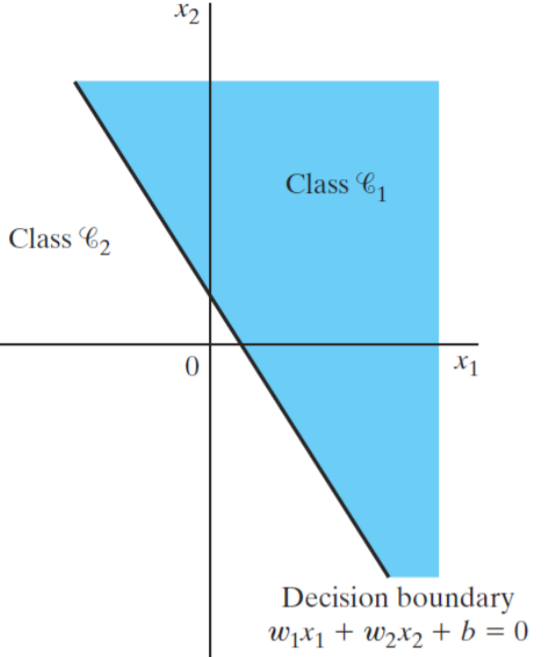
\includegraphics[height=6cm]{example_linear_classifier.PNG}
    \caption{The decision boundary (line) separates the $x_1,x_2$ space in two semi-planes.}
    %\label{fig:my_label}
\end{figure}

\subsection{Its architecture}

The perceptron takes as input a bunch of data $\textbf{x}^1, \textbf{x}^2, \ldots , \textbf{x}^n$ and outputs a \emphasis{label} value $y \in \{0,1\}$ for each, which indicates the predicted class where the data sample belongs. Let's analyse the architecture in 2D.

The inputs are $x_1, x_2$. $x_1$ is weighted (multiplied) by some value $x_1$ and $x_2$ by $w_2$. The perceptron also needs some bias so that the decision boundary doesn't always cross the origin. This can be considered as an additional input $x_0 = 1$, multiplied by weight $w_0$. Their weighted sum $S=x_1w_1 + x_2w_2 + b$ is evaluated and passed through an \emphasis{activation} function $f$, whose value determines the input's class, so the final predicted output is:
\begin{equation}
    y_{pred} =  f(x_1w_1 + x_2w_2 + b)
\end{equation}
Using the dot product, this can be written more compactly as:
\begin{equation}
    y_{pred} =  f(\textbf{w} \cdot \textbf{x} + b)
\end{equation}
$\textbf{w}$ is the \emphasis{weight vector} and $b$ (a scalar) the \emphasis{bias}. A simple activation function $f$ is the \emphasis{step function}.
\begin{definition}
The \emphasis{step function} is defined as
\begin{equation}
    f(x) = \left\{
\begin{array}{ll}
      1, & x\geq 0 \\
      0, & x<0\\
\end{array} \right.
\end{equation}
\end{definition}
So for our model the predicted output $f(\textbf{w} \cdot \textbf{x} + b) \in \{0,1\}$ depends simply on the sign of $\textbf{w} \cdot \textbf{x} + b$. In 2D, for positive instances we have $w_1x_1 + w_2x_2 + b \geq 0$ and for negative ones $w_1x_1 + w_2x_2 + b < 0$. 
\begin{figure}[H]
    % ref https://trevorcohn.github.io/comp90051-2017/slides/06_vectors_perceptron.pdf
    \centering
    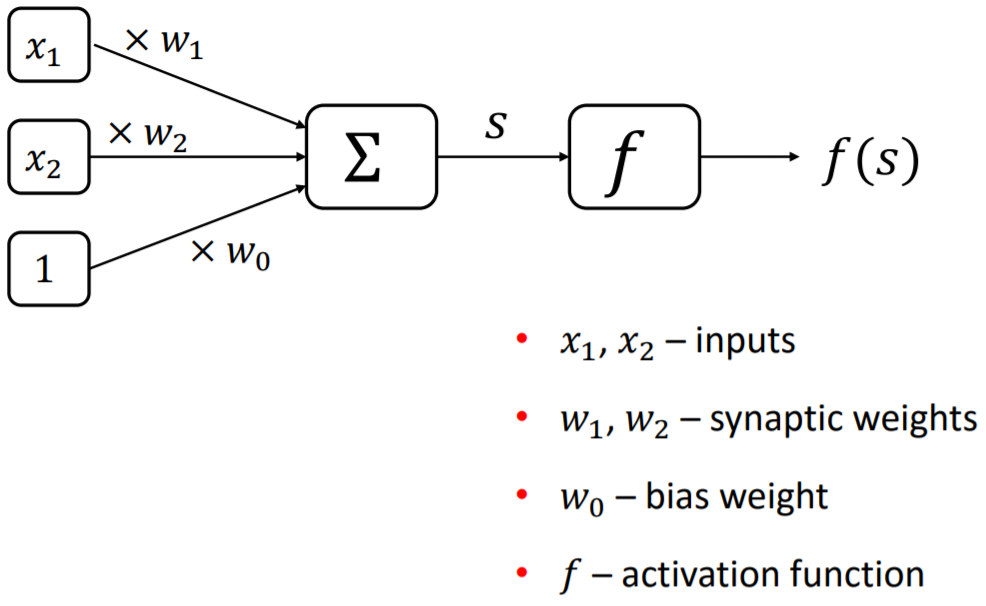
\includegraphics[height=5cm]{perceptron_architecture.png}
    \caption{Perceptron model.}
    %\label{fig:my_label}
\end{figure}
% ref https://ocw.mit.edu/courses/health-sciences-and-technology/hst-947-medical-artificial-intelligence-spring-2005/lecture-notes/ch7_mach3.pdf
So the goal of the perceptron is for each data point $\textbf{x}\in \mathbb{R}^n$ find some $\textbf{w}\in \mathbb{R}^n$ and an offset $b\in \mathbb{R}$ such that it can correctly decide whether $\textbf{w}\cdot \textbf{x} + b \geq 0$ or  $\textbf{w}\cdot \textbf{x} + b < 0$. Therefore if the number of features of the input is $n$ (e.g. 2 in the 2D space) then the number of coefficients to be learned is $n+1$ (e.g. $w_0,\ w_1,\ b$ for the 2D space). The \emphasis{decision boundary} is a line for 2D inputs, a plane for 3D, etc., and in general it's called \emphasis{hyperplane}.
\begin{definition}
The equation of the decision boundary hyperplane is 
\begin{equation}
    \textbf{w}\cdot \textbf{x} + b = 0
\end{equation}
or equivalently
\begin{equation}
    \sum\limits_{i=1}^{n}{w_ix_i} + b = 0
\end{equation}
$w_i$ and $b$ are to be learned.
\end{definition}

\subsection{Perceptron for logical operations}

\subsubsection{AND perceptron}
The perceptron can be used to classify samples $\textbf{x}=(x_1,x_2)$ for which the output is defined by the AND operation, as given by the following truth table.
\begin{center}
\begin{tabular}{c|c|c}
$x_1$ & $x_2$ & $y$ \\
\hline
0 & 0 & 0 \\
0 & 1 & 0 \\
1 & 0 & 0 \\
1 & 1 & 1 
\end{tabular}
\end{center}
We therefore want for the predicted output:
\begin{gather*}
f(0,0) = 0 \Rightarrow 0\cdot w_1 + 0\cdot w_2 + b < 0 \tag{1}\\
f(0,1) = 0 \Rightarrow 0\cdot w_1 + 1\cdot w_2 + b < 0 \tag{2}\\
f(1,0) = 0 \Rightarrow 1\cdot w_1 + 0\cdot w_2 + b < 0 \tag{3}\\
f(1,1) = 1 \Rightarrow 1\cdot w_1 + 1\cdot w_2 + b > 0 \tag{4}
\end{gather*}
A set of weights that satisfies Eq. (1)-(4) is $w_1=1,\ w_2=1,\ b=-1.3$. Therefore in 2D space the inputs would be mapped in two classes as follows. 
\begin{figure}[H]
    \centering
    %%% Notes:
% Make sure that the line label is in the correct position:
% (axis cs: x, y) -- (axis cs: x, y)


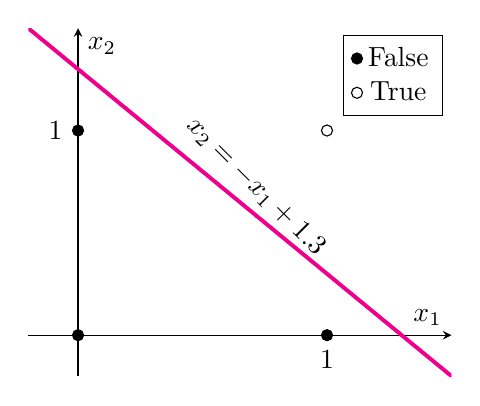
\begin{tikzpicture}

\begin{axis}[
    height=6cm,
    axis lines=middle,
    xmin=-0.2, xmax=1.5,
    ymin=-0.2, ymax=1.5,
    xtick={0,1}, ytick={0,1},
    xlabel=$x_1$, ylabel=$x_2$
]
%-----------------------------------------------------
% points
\addplot [only marks] table {
    0 0
    0 1
    1 0
};
\addplot [only marks, mark=o] table {
    1 1
};
%-----------------------------------------------------
% straight line
\addplot [domain=-10:10, samples=2, solid, color=magenta, line width=.5mm] {-x + 1.3};
\draw [ultra thick] 
        (axis cs: 0.65 ,0.65) -- (axis cs: 0.65 ,0.65)
        node[pos=0.5, above, rotate=-45] {$x_2 = -x_1 + 1.3$};
%-----------------------------------------------------
% legend
\addlegendentry{False}
\addlegendentry{True}

\end{axis}

\end{tikzpicture}

    \caption{Boundary line for prediction $y=x_1 \ \textup{AND} \ x_2$.}
    %\label{fig:my_label}
\end{figure}
A good boundary line that separates the data in two classes is $x_2 = -x_1 + 1.3$ (the weights and offset were found from Eq. (1)-(4)).
The semi-plane for which the prediction is TRUE, i.e. $y=1$, is:
\begin{gather*}
   x_1 + x_2 - 1.3 \geq 0 \Rightarrow\\
   1\cdot x_1 + 1\cdot x_2 + (-1.3) = 0
\end{gather*}
Therefore the data can be classified by an perceptron with $w_1=1, \ w_2 = 1, \ b = -1.3$.

\subsubsection{OR perceptron}
Similarly, for the OR truth table and boundary line we have:
\begin{multicols}{2}
\begin{center}
\begin{tabular}{c|c|c}
$x_1$ & $x_2$ & $y$ \\
\hline
0 & 0 & 0 \\
0 & 1 & 1 \\
1 & 0 & 1 \\
1 & 1 & 1 
\end{tabular}
\end{center}
\columnbreak
\begin{figure}[H]
    \centering
    %%% Notes:
% Make sure that the line label is in the correct position:
% (axis cs: x, y) -- (axis cs: x, y)


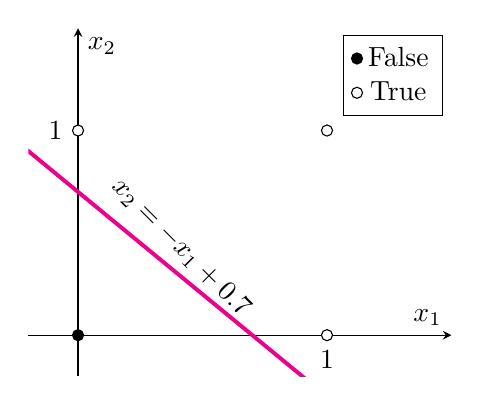
\begin{tikzpicture}

\begin{axis}[
    height=6cm,
    axis lines=middle,
    xmin=-0.2, xmax=1.5,
    ymin=-0.2, ymax=1.5,
    xtick={0,1}, ytick={0,1},
    xlabel=$x_1$, ylabel=$x_2$
]
%-----------------------------------------------------
% points
\addplot [only marks] table {
    0 0
};
\addplot [only marks, mark=*, mark options={solid,fill=white}] table {
    0 1
    1 0
    1 1
};
%-----------------------------------------------------
% straight line
\addplot [domain=-10:10, samples=2, solid, color=magenta, line width=.5mm] {-x + 0.7};
\draw [ultra thick] 
        (axis cs: 0.35 ,0.35) -- (axis cs: 0.35 ,0.35)
        node[pos=0.5, above, rotate=-45] {$x_2 = -x_1 + 0.7$};
%-----------------------------------------------------
% legend
\addlegendentry{False}
\addlegendentry{True}

\end{axis}

\end{tikzpicture}

    \caption{Boundary line for prediction $y=x_1 \ \textup{OR} \ x_2$.}
    %\label{fig:my_label}
\end{figure}
\end{multicols}
For the prediction $y=1$ (TRUE) we have:
\begin{gather*}
   x_1 + x_2 - 0.7 \geq 0 \Rightarrow\\
   1\cdot x_1 + 1\cdot x_2 + 0.7 = 0
\end{gather*}
Therefore the perceptron weights are $w_1=1, \ w_2 = 1, \ b = -0.7$.

\subsubsection{NOT perceptron}
The NOT operation is slightly different from the other two as it's defined for only one input and doesn't care about the other. Let's try to design a perceptron for $y=NOT(x_2)$. In the following truth table, X stands for ``don't care''.
\begin{multicols}{2}
\begin{center}
\begin{tabular}{c|c|c}
$x_1$ & $x_2$ & $y$ \\
\hline
X & 0 & 1 \\
X & 1 & 0
\end{tabular}
\end{center}
\columnbreak

\begin{figure}[H]
    \centering
    %%% Notes:
% Make sure that the line label is in the correct position:
% (axis cs: x, y) -- (axis cs: x, y)


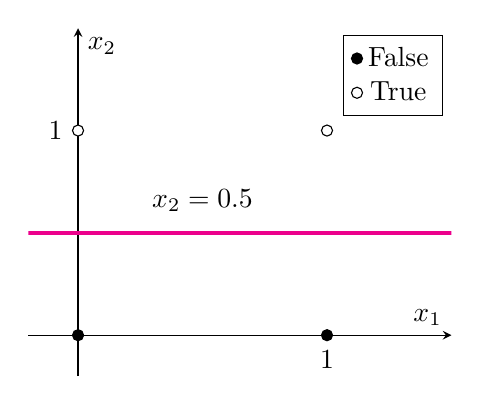
\begin{tikzpicture}

\begin{axis}[
    height=6cm,
    axis lines=middle,
    xmin=-0.2, xmax=1.5,
    ymin=-0.2, ymax=1.5,
    xtick={0,1}, ytick={0,1},
    xlabel=$x_1$, ylabel=$x_2$
]
%-----------------------------------------------------
% points
\addplot [only marks] table {
    1 0
    0 0
};
\addplot [only marks, mark=*, mark options={solid,fill=white}] table {
    0 1
    1 1
};
%-----------------------------------------------------
% straight line
\addplot [domain=-10:10, samples=2, solid, color=magenta, line width=.5mm] {0.5};
\draw [ultra thick] 
        (axis cs: 0.5 ,0.55) -- (axis cs: 0.5 ,0.55)
        node[pos=0.5, above, rotate=0] {$x_2 = 0.5$};
%-----------------------------------------------------
% legend
\addlegendentry{False}
\addlegendentry{True}

\end{axis}

\end{tikzpicture}

    \caption{Boundary line for prediction $y=x_1 \ \textup{NOT} \ x_2$.}
    %\label{fig:my_label}
\end{figure}
\end{multicols}


\subsubsection{XOR perceptron}
For the XOR operation, the truth table and output is:
\begin{multicols}{2}
\begin{center}
\begin{tabular}{c|c|c}
$x_1$ & $x_2$ & $y$ \\
\hline
0 & 0 & 0\\
0 & 1 & 1\\
1 & 0 & 1\\
1 & 1 & 0
\end{tabular}
\end{center}

\columnbreak
\begin{figure}[H]
    \centering
    %%% Notes:
% Make sure that the line label is in the correct position:
% (axis cs: x, y) -- (axis cs: x, y)


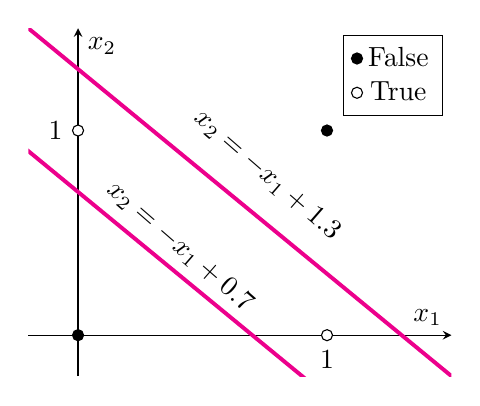
\begin{tikzpicture}

\begin{axis}[
    height=6cm,
    axis lines=middle,
    xmin=-0.2, xmax=1.5,
    ymin=-0.2, ymax=1.5,
    xtick={0,1}, ytick={0,1},
    xlabel=$x_1$, ylabel=$x_2$
]
%-----------------------------------------------------
% points
\addplot [only marks] table {
    0 0
    1 1
};
\addplot [only marks, mark=*, mark options={solid,fill=white}] table {
    0 1
    1 0
};
%-----------------------------------------------------
% straight line
\addplot [domain=-10:10, samples=2, solid, color=magenta, line width=.5mm] {-x + 0.7};
\draw [ultra thick] 
        (axis cs: 0.35 ,0.35) -- (axis cs: 0.35 ,0.35)
        node[pos=0.4, above, rotate=-41] {$x_2 = -x_1 + 0.7$};
        
\addplot [domain=-10:10, samples=2, solid, color=magenta, line width=.5mm] {-x + 1.3};
\draw [ultra thick] 
        (axis cs: 0.7 ,0.7) -- (axis cs: 0.7 ,0.7)
        node[pos=0.4, above, rotate=-41] {$x_2 = -x_1 + 1.3$};
        
%-----------------------------------------------------
% legend
\addlegendentry{False}
\addlegendentry{True}

\end{axis}

\end{tikzpicture}

    \caption{XOR outputs and the two boundary lines needed to classify them.}
    \label{fig:xor_input_output}
\end{figure}

\end{multicols}
However, the is \textit{no single boundary line} that can correctly separate the data. Two lines are needed as shown in \ref{fig:xor_input_output}. The area we want to classify as $y=1$ is desribed by:
\begin{gather*}
x_1 + x_2 -0.7 \geq 0 \;\; \textup{and} \;\; x_1 + x_2 -1.3 <0 \Rightarrow\\
(x_1 \; OR \; x_2) \;\; AND \;\; \left(NOT \;\; (x_1 \; AND \; x_2)\right)
\end{gather*}
Schematically, the XOR perceptron is described as follows:
\begin{figure}[H]
    \centering
    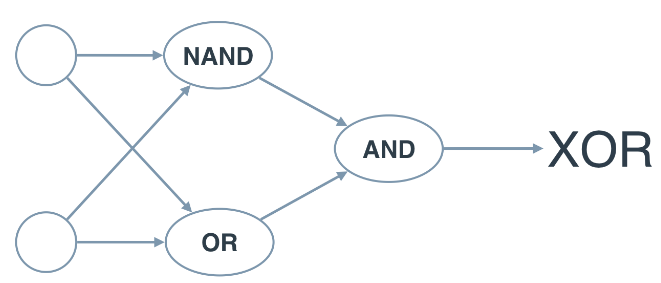
\includegraphics[height=4cm]{xor_multiplayer.PNG}
    \caption{XOR design as a combination of other perceptrons.}
    %\label{fig:my_label}
\end{figure}


\subsubsection{Linear separability}

Linear separability means that the two input classes $X_0,\ X_1$ can be perfectly separated by a straight line. Mathematically, this is expressed as:
\begin{definition}
Let $X_0,\ X_1$ be two disjoint sets of the $n$-dimensional input data $X$. Then the sets are linearly separable if there exist $n+1$ real numbers $w_0,\ w_1, \ldots, w_{n-1}, b$ such that:
    \begin{gather}
      \sum_{i=1}^{n}{w_ix_i} - b > 0 \quad \forall x \in X_0  \quad \textup{and}\\
      \sum_{i=1}^{n}{w_ix_i} - b < 0 \quad \forall x \in X_1
    \end{gather}
\end{definition}


\subsection{The perceptron trick - intuition}
When a point is classified there are 3 possibilities:
\begin{enumerate}
    \item It is correctly classified, i.e. $y = y_{pred}$.
    \item A positive sample is misclassified, i.e. $y=1$ and $y_{pred}=0$.
    \item A negative sample is misclassified, i.e. $y=0$ and $y_{pred}=1$.
\end{enumerate}
For every misclassfied point, the weights $w_1,\ w_2$ and bias $b$ need to be corrected. Before describing the perceptron correction trick, the maths of the hyperplane needs to be understood. For simplicity, we'll consider the hyperplane as a line but the observations below can be generalised.
\begin{corollary}
For the boundary line $w_1x_1 + w_2x_2 + b = 0$, The vector $\textbf{w} = (w_1,w_2)$ is perpendicular to it.
\end{corollary}
\begin{corollary} \label{cor:dist_from_origin}
For the boundary line $w_1x_1 + w_2x_2 + b = 0$, its distance from the origin is $\frac{b}{\left|\left|\textbf{w}\right|\right|}$.
\end{corollary}
\begin{proof}
\quad \\
See \ref{app:min_dist_origin}.
\end{proof}
% ref https://www.cs.utah.edu/~piyush/teaching/8-9-print.pdf
Denoting negative instances as $y=0$ and positive as $y=1$, the perceptron update trick is based on the following heuristic that handles false cases.
\begin{itemize}
    \item $y=1$ but the perceptron thinks that $y_{pred} = 0 \Rightarrow \textbf{w}_{old}\textbf{x} + b_{old} < 0$.
    
    Then the updates should be
        \begin{gather*}
            \textbf{w}_{new} = \textbf{w}_{old} + \textbf{x} \\
            b_{new} = b_{old} + 1
        \end{gather*}
        
    Indeed, in this case for the output of the new updates we have
    \[
    \begin{split}
        \textbf{w}_{new}\cdot \textbf{x} + b_{new} 
        &= \left( \textbf{w}_{old} + \textbf{x} \right)\textbf{x} + b_{old} + 1\\
        &=\textbf{w}_{old}\cdot \textbf{x} + b_{old} + \textbf{x} \cdot \textbf{x} + 1\\
        &>  \textbf{w}_{old}\cdot \textbf{x} + b_{old}
    \end{split}
    \]
    Therefore the updated sum is more positive than the old, hence has better chance of being classified correctly by the step function. Geometrically, this  effect is illustated for the line below, for which $b=0$ for simplicity so the effect on the offset is not demonstrated. 
    \begin{figure}[H]
        \centering
        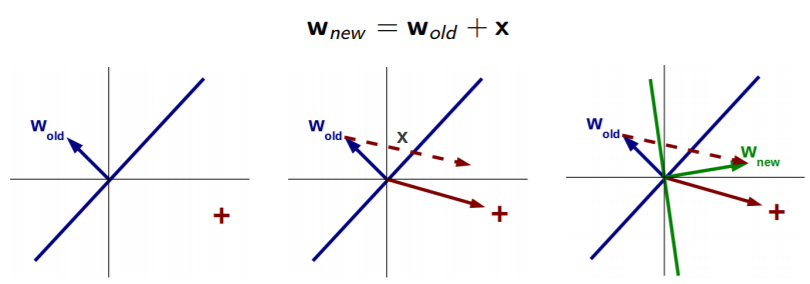
\includegraphics[scale=0.75]{img/line_pos_correction.PNG}
        \caption{Correction of actual positive misclassified instance.}
        %\label{fig:my_label}
    \end{figure}
    For $b=0$, to classify a point $x$ as positive, we simply want $\textbf{w}\cdot \textbf{x}>0$, i.e. the angle between $x$ and $b$ to be acute. So in this case the weight vector should point towards positive instances. 
    
    \item $y=0$ but the perceptron thinks that $y_{pred} = 1 \Rightarrow \textbf{w}_{old}\textbf{x} + b_{old} > 0$. 
    
    Then the weights and offset are corrected by
            \begin{gather*}
            \textbf{w}_{new} = \textbf{w}_{old} - \textbf{x} \\
            b_{new} = b_{old} - 1
        \end{gather*}
    Indeed, in this case for the new output
        \[
    \begin{split}
        \textbf{w}_{new}\cdot \textbf{x} + b_{new} 
        &= \left( \textbf{w}_{old} - \textbf{x} \right)\textbf{x} + b_{old} - 1\\
        &=\textbf{w}_{old}\cdot \textbf{x} + b_{old} - \textbf{x} \cdot \textbf{x} - 1\\
        &<  \textbf{w}_{old}\cdot \textbf{x} + b_{old}
    \end{split}
    \]
    The new output is more negative than the old, as desired. Below is how the correction works geometrically (again, for $b=0$).
        \begin{figure}[H]
        \centering
        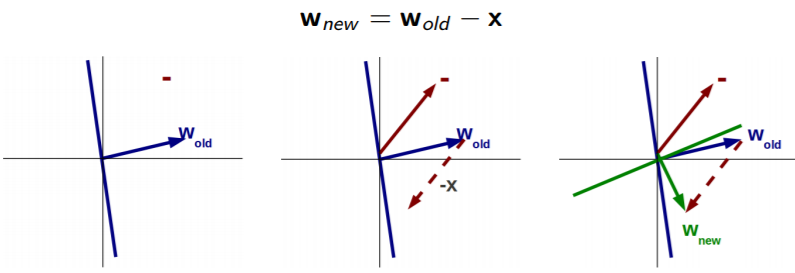
\includegraphics[scale=0.75]{img/line_neg_correction.PNG}
        \caption{Correction of actual negative misclassified instance.}
        %\label{fig:my_label}
    \end{figure}
    Similarly, for $b=0$, to classify a point $\textbf{x}$ as negative we want $\textbf{w}\cdot \textbf{x} < 0$, i.e. the angle between $\textbf{x}$ and $\textbf{b}$ to be obtuse, i.e. the weight vector to point away from negative instances, as shown in the correction.
\end{itemize}


\subsection{Perceptron weight correction - the algorithm}

In reality, the weights and bias are not updated by $\textbf{x}$ and $1$ as this is too large and causes predicition errors to the other measurements, but by small fractions of them.
\begin{definition}
The perceptron correction weight updates are
\begin{gather}
    \textbf{x}_{new} = \textbf{w}_{old} + \eta\ \textbf{x}\\
    b_{new} = b_{old} + \eta
\end{gather}
$\eta$ is called the \emphasis{learning rate}.
\end{definition}
\begin{exmp}
We have the decision line $3x_1+4x_2-10=0$ and the positive point $\textbf{x}=(1,1)$ that is misclassified. If the learning rate is $\eta=0.1$, how many iterations will it take to correct it? (Credits: Udacity, \TODO)
\end{exmp}
\begin{soln}
Since the point to correct is $(4,5)$ and is actually negative ($y=0)$, after one update we sum and the coefficients are
\begin{gather*}
    w_1^{(1)} = 3 + 1\ \eta\\
    w_2^{(1)} = 4 + 1\ \eta \\
    b^{(1)} = -10 + \eta
\end{gather*}
And after $n$ updates they are:
\begin{gather*}
    w_1^{(n)} = 3 +  n\ \eta = 3+0.1n\\
    w_2^{(n)} = 4 + n \ \eta = 4+0.1n \\
    b^{(n)} = -10 + n\ \eta  = -10+0.1n
\end{gather*}
We want to keep correcting until:
\begin{gather}
    1 w_1^{(n)} + 1 w_2^{(n)} - 10 + 0.1n > 0 \Rightarrow\\
    3+0.1n + 4+0.1n- 10+0.1n > 0 \Rightarrow \\
    n > 10
\end{gather}
So at least 10 itearations are required to correct it.
\end{soln}
That is the basis of the perceptron algorithm -- iterate for each point, and if it is misclassified, update accordingly. It is described in pseudocode below. It can be proved that for linearly separable data the algorithm is guaranteed to converge.
\begin{algorithm}[H]
\caption{The final perceptron algorithm.}
\begin{algorithmic}[1]
\Procedure{Perceptron} {$\textbf{x}_{1\times m},\;\textbf{y}_{1\times m},\; \eta, \; N_{epochs}$}
\State \Comment{$\textbf{x}$: a list of $m$ vectors (input data), $\textbf{y}$: label (0 or 1) for each input. Each input also has $n$ features.}
\State \Comment{$\eta$: learning rate, $N_{epochs}$: how many epochs (iterations) we want the algorithm to run for.}
\State $w_1,\ w_2, \ \ldots, \ w_n,\ b \leftarrow$ random values
\For {$i=0,\ldots,N_{epochs}$}
\For{$j=1,\ldots,m$}
\If {$y_j=0$ and $\textbf{w}\cdot \textbf{x}_j + b > 0$} \Comment{misclassified negative point}
\State $\textbf{w} \leftarrow \textbf{w} - \eta \ \textbf{x}_j$
\State $b \leftarrow b - \eta$
\ElsIf {$y_j=1$ and $\textbf{w}\cdot \textbf{x}_j + b < 0$} \Comment{misclassified positive point}
\State $\textbf{w} \leftarrow \textbf{w} + \eta \ \textbf{x}_j$
\State $b \leftarrow b + \eta$
\EndIf
\EndFor
\EndFor
\State \textbf{return} $\textbf{w}$, $b$
\EndProcedure
\end{algorithmic}
\end{algorithm}


\subsection{Algorithm implementation}

An implementation that learns the weights online (updates them as it reads the data) and runs for a certain number of epochs is listed in \ref{app:perc_algo_src}. It is based on Udacity's skeleton code. In Fig. \ref{fig:perc_training_out}, where its result is visualised, the final boundary line is solid and the updates are dashed.
\begin{figure}[H]
    \centering
    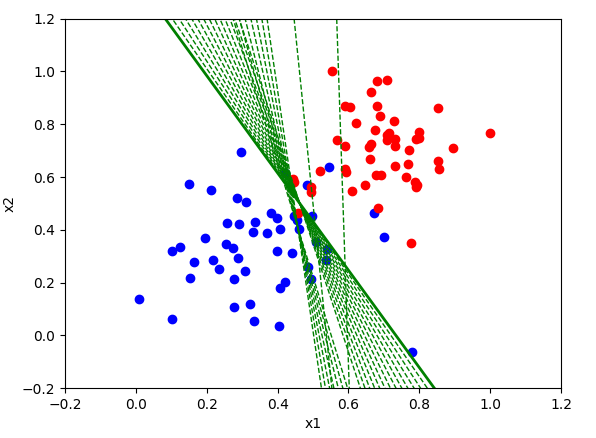
\includegraphics[height=5.5cm]{img/algo_training_out.PNG}
    \caption{Online training results for percetron online training. Positive data are blue and negative red.}
    \label{fig:perc_training_out}
\end{figure}


% http://130.243.105.49/~lilien/ml/seminars/2007_02_01b-Janecek-Perceptron.pdf !!
% line maths: *** https://stats.stackexchange.com/questions/143895/a-challenge-with-linear-classification-and-distance-to-origin, *** https://math.stackexchange.com/questions/1029153/deriving-the-normal-distance-from-the-origin-to-the-decision-surface !!, *** https://en.wikipedia.org/wiki/Distance_from_a_point_to_a_line !!



% https://web.archive.org/web/20181003041048/https://www.cs.utah.edu/~zhe/pdf/lec-10-perceptron-upload.pdf, https://trevorcohn.github.io/comp90051-2017/slides/06_vectors_perceptron.pdf, http://mr-pc.org/t/cse5526/pdf/01b-perceptron.pdf, http://www.cs.umd.edu/class/spring2018/cmsc422-0101/slides0201/lecture_07.pdf
%

%=-=-=-=-=-=-=-=-=-=-=-=-=-=-=-=-=-=-=-=-=-=-=-=-=-=-=-=-=-=-=-=-=-=-=-=-=-=-=-=-
% Appendices
%=-=-=-=-=-=-=-=-=-=-=-=-=-=-=-=-=-=-=-=-=-=-=-=-=-=-=-=-=-=-=-=-=-=-=-=-=-=-=-=-
\newpage
\appendix

\section{Appendices}

% ------------------------ New appendix ------------------------ %
\newpage
\subsection{Proof of Cor. \ref{cor:dist_from_origin} (perceptron boundary line)}
\label{app:min_dist_origin}

% another proof: https://math.stackexchange.com/a/1948344
The decision boundary has equation
\[
w_1x_1 + w_2x_2 + b = 0 \tag{1}
\]
$\textbf{x}$ is a vector from the origin to some point $(x_1,x_2)$ on the line. We are looking to minimise $\left|\left| \textbf{x}\right|\right|$ under condition (1), where $\textbf{x}=(x_1,x_2)$. Eq. (1) can be re-written as:
\[
\textbf{w}\cdot \textbf{x} = -b \tag{2}
\]
, where $\textbf{w}\cdot \textbf{x} = \left|\left| \textbf{w}\right|\right| \left|\left| \textbf{x}\right|\right|cos\left(\theta \right)$ is the dot product, $\theta$ the angle between the two vectors, and $w=(w_1,w_2)$ the weight vector perpendicular to the line. Therefore, and since $\left|\left|x\right| \right|\geq 0$,  Eq. (2) can be solved for $\left|\left|x\right| \right|$ as:
\begin{gather*}
\left|\left|\textbf{x}\right| \right| =  \frac{\left|b\right|}{\left|\left|\textbf{w} \right| \right| \left|\cos(\theta)\right |} \Rightarrow \\
\left|\left|\textbf{x}\right| \right| \leq \frac{\left|b\right|}{\left|\left|\textbf{w} \right| \right|}
\end{gather*}
The equality is achieved when $\left| \cos(\theta) \right|= 1$, i.e. when $\textbf{x}$ and $\textbf{w}$ are parallel or anti-parallel. The minimum distance of $\textbf{x}$ from the origin is therefore $\frac{\left|b\right|}{\left|\left|\textbf{w} \right| \right|}$.\qed


% ------------------------ New appendix ------------------------ %
\newpage
\subsection{Perceptron with online training in Python.}
\label{app:perc_algo_src}
\inputminted{python}{src/perceptron.py}

%=-=-=-=-=-=-=-=-=-=-=-=-=-=-=-=-=-=-=-=-=-=-=-=-=-=-=-=-=-=-=-=-=-=-=-=-=-=-=-=-
% References
%=-=-=-=-=-=-=-=-=-=-=-=-=-=-=-=-=-=-=-=-=-=-=-=-=-=-=-=-=-=-=-=-=-=-=-=-=-=-=-=-
\newpage
\printbibliography


\end{document}